\documentclass[11pt,a4paper]{article}

% ========== Preamble ==========
\usepackage[utf8]{inputenc}
\usepackage[T1]{fontenc}
\usepackage{amsmath,amssymb,amsthm}
\usepackage[margin=2.5cm]{geometry}
\usepackage{xcolor}
\usepackage{tcolorbox}
\usepackage{booktabs}
\usepackage{enumitem}
\usepackage{array}
\usepackage{titlesec}
\usepackage{fancyhdr}
\usepackage{graphicx}
\usepackage{tikz}
\usetikzlibrary{arrows.meta,positioning,calc,shapes.geometric,fit}

% Hyperref last
\usepackage[
    colorlinks=true,
    linkcolor=blue!70!black,
    citecolor=darkgray,
    urlcolor=blue!70!black,
    bookmarks=true,
    bookmarksnumbered=true,
    unicode=true
]{hyperref}

% ========== Page style ==========
\pagestyle{fancy}
\fancyhf{}
\setlength{\headheight}{14pt}
\fancyhead[L]{\small Trik Sulap Kartu --- Penjelasan Matematis}
\fancyhead[R]{\small \thepage}
\renewcommand{\headrulewidth}{0.4pt}

% ========== Section styling ==========
\titleformat{\section}{\Large\bfseries\color{blue!50!black}}{\thesection}{1em}{}
\titleformat{\subsection}{\large\bfseries\color{blue!40!black}}{\thesubsection}{1em}{}

% ========== Custom theorem envs ==========
\theoremstyle{definition}
\newtheorem{definisi}{Definisi}[section]
\newtheorem{teorema}{Teorema}[section]
\newtheorem{lemma}[teorema]{Lemma}

% ========== Custom tcolorbox styles ==========
\newtcolorbox{rumusbox}[1][]{
    colback=blue!5,
    colframe=blue!50!black,
    fonttitle=\bfseries,
    title=#1,
    boxrule=0.8pt,
    arc=3pt,
    left=8pt,right=8pt,top=6pt,bottom=6pt
}

\newtcolorbox{insightbox}[1][]{
    colback=amber!10,
    colframe=orange!70!black,
    fonttitle=\bfseries,
    title=#1,
    boxrule=0.8pt,
    arc=3pt,
    left=8pt,right=8pt,top=6pt,bottom=6pt
}

% workaround: amber not defined, use orange
\definecolor{amber}{rgb}{1.0, 0.7, 0.0}

\newtcolorbox{tahapbox}[1][]{
    colback=gray!5,
    colframe=gray!50!black,
    fonttitle=\bfseries\color{white},
    coltitle=white,
    title=#1,
    boxrule=0.6pt,
    arc=3pt,
    left=8pt,right=8pt,top=6pt,bottom=6pt
}

% ========== Title metadata ==========
\title{\bfseries\LARGE Trik Sulap Kartu 2$\heartsuit$ \\[0.3em]
       \large Penjelasan Matematis Lengkap --- dari Kocok sampai Teman Tahu Kartumu}
\author{}
\date{}

% ========== Hypersetup ==========
\hypersetup{
    pdftitle={Trik Sulap Kartu - Penjelasan Matematis},
    pdfauthor={Z.ai},
    pdfsubject={Matematika Diskrit, Teori Himpunan, Algoritma Deterministik},
    pdfkeywords={sulap kartu, set difference, konvergensi, deterministik, 27-card trick}
}

\begin{document}

\maketitle
\thispagestyle{empty}

\begin{abstract}
\noindent
Dokumen ini membongkar secara matematis bagaimana seorang temanmu dapat mengetahui dengan pasti kartu yang kamu pilih (misalnya 2$\heartsuit$) dari sebuah deck poker standar berisi 52 kartu, meskipun kamu mengocoknya secara acak. Penjelasan dibagi dalam dua mekanisme matematis yang berbeda: (1) \emph{Metode Selisih Himpunan} yang merupakan cara langsung dan paling sederhana --- temanmu cukup memeriksa 51 kartu yang ia pegang dan menemukan kartu mana dari deck standar yang tidak ada; dan (2) \emph{Metode Konvergensi Algoritmik} via pembagian tumpukan berulang yang merupakan trik sulap klasik ``27-Card Trick''. Kedua metode bersifat \textbf{deterministik} --- tidak ada unsur keberuntungan, hanya pemetaan matematis pada himpunan terbatas.
\end{abstract}

\vspace{0.5em}

\tableofcontents
\newpage

% =====================================================================
\section{Skenario Lengkap: dari Kocok sampai Teman Tahu Kartumu}
% =====================================================================

Sebelum membahas rumus, mari kita pahami persis alur peristiwanya seperti yang kamu alami. Skenario ini penting karena setiap langkah punya peran matematis yang berbeda:

\begin{tahapbox}[Tahap 1 --- Kamu mengocok 52 kartu]
Kamu memegang sebuah deck poker standar berisi 52 kartu yang sudah campur aduk. Pengocokan ini murni acak --- tidak ada urutan tertentu, tidak ada pola, tidak ada konspirasi. Dalam istilah probabilitas, ini adalah \emph{uniform random permutation} dari 52 kartu.
\end{tahapbox}

\begin{tahapbox}[Tahap 2 --- Kamu menyerahkan deck ke teman]
Setelah selesai mengocok, kamu memberikan seluruh tumpukan ke temanmu. Pada titik ini, temanmu memegang deck lengkap 52 kartu.
\end{tahapbox}

\begin{tahapbox}[Tahap 3 --- Kamu disuruh memilih satu kartu secara acak]
Temanmu menyodorkan deck (yang masih dalam keadaan tertutup) dan menyuruh kamu mengambil satu kartu. Kamu tidak tahu apa yang kamu ambil --- mungkin 2$\heartsuit$, mungkin K$\spadesuit$, mungkin apa saja. Kamu mengambil satu, melihatnya sendiri (misalnya 2$\heartsuit$), lalu menyimpannya. Kamu tidak menunjukkan ke temanmu.
\end{tahapbox}

\begin{tahapbox}[Tahap 4 --- Kamu mengocok lagi]
Setelah mengambil kartu pilihanmu, kamu (atau temanmu) mengocok sisa deck lagi. Pengocokan ini juga murni acak --- tidak ada pola.
\end{tahapbox}

\begin{tahapbox}[Tahap 5 --- Temanmu memisah-misahkan deck jadi beberapa bagian]
Temanmu mulai membagi sisa deck menjadi beberapa tumpukan kecil (misalnya 3 tumpukan). Pembagian ini terlihat seperti bagian dari trik sulap.
\end{tahapbox}

\begin{tahapbox}[Tahap 6 --- Temanmu bertanya: ``Apakah kartu kamu ada di bagian ini?'']
Untuk setiap tumpukan, temanmu menunjukinya ke kamu dan bertanya: ``Apakah kartu kamu ada di tumpukan ini?'' Kamu menjawab ``Ya'' atau ``Tidak'' dengan jujur.
\end{tahapbox}

\begin{tahapbox}[Tahap 7 --- Berlanjut sampai tersisa 3 kartu]
Temanmu mengulang proses bagi-tumpukan-dan-tanya beberapa kali. Setiap kali kamu bilang ``Ya'', temanmu mengambil tumpukan itu sebagai deck baru. Setelah beberapa ronde, tersisa 3 kartu. Dan kartu kamu PASTI ada di antara 3 itu.
\end{tahapbox}

Pertanyaan kunci: \textbf{Bagaimana temanmu tahu kartumu adalah 2$\heartsuit$?} Dua jawaban matematis akan diberikan di bab berikut.

% =====================================================================
\section{Notasi Matematis Dasar}
% =====================================================================

Sebelum masuk ke rumus, mari kita tetapkan notasi yang dipakai sepanjang dokumen.

\begin{definisi}[Deck Standar]
Deck poker standar adalah himpunan
\[
\mathcal{D} = \{ c_1, c_2, c_3, \ldots, c_{52} \}, \quad |\mathcal{D}| = 52,
\]
di mana setiap $c_i$ adalah pasangan (rank, suit) unik. Rank ada 13 macam ($A, 2, 3, \ldots, K$) dan suit ada 4 macam ($\heartsuit, \diamondsuit, \clubsuit, \spadesuit$), sehingga $13 \times 4 = 52$ kartu unik.
\end{definisi}

\begin{definisi}[Kartu Pilihan User]
Misalkan kamu memilih satu kartu tertentu, sebut saja $c^* \in \mathcal{D}$. Dalam contoh kamu, $c^* = 2\heartsuit$. Nilai $c^*$ tidak diketahui temanmu di awal --- ini yang harus ia temukan.
\end{definisi}

\begin{definisi}[Sisa Deck yang Dimiliki Teman]
Setelah kamu mengambil $c^*$ dan menyimpannya, temanmu memegang sisa deck:
\[
\mathcal{R} = \mathcal{D} \setminus \{c^*\}, \quad |\mathcal{R}| = 51.
\]
Himpunan $\mathcal{R}$ inilah yang temanmu \emph{pegang dan lihat}.
\end{definisi}

\begin{definisi}[Operasi Selisih Himpunan]
Operasi selisih himpunan (set difference) $\setminus$ didefinisikan sebagai:
\[
A \setminus B = \{ x \in A \mid x \notin B \}.
\]
Secara intuitif: ``ambil semua elemen $A$, buang yang juga ada di $B$''.
\end{definisi}

% =====================================================================
\section{Metode 1: Selisih Himpunan --- Cara Asli Temanmu}
% =====================================================================

\subsection{Ide Dasar}

Inilah kunci yang sering tidak disadari: temanmu \textbf{tidak perlu} membagi-bagi tumpukan untuk tahu kartumu. Dari obrolan WhatsApp yang kamu lampirkan, temanmu sendiri mengaku:

\begin{quote}
\textit{``tanpa gua bagi2 in gua juga bisa langsung tau kartu lu''} \\
\textit{``langsung gua bagi semua (kecuali kartu lu) misalnya, itu juga bisa''} \\
\textit{``cuma kan bagi2 itu buat some kind of playing aja biar gak langsung selesai sulapnya''}
\end{quote}

Pernyataan ini \textbf{sangat jujur secara matematis}. Temanmu tidak berbohong. Trik sebenarnya sangat sederhana: \textbf{dia tahu kartumu dengan menghitung selisih antara deck standar dengan sisa kartu yang ia pegang}.

\subsection{Rumus Inti}

Karena $\mathcal{D}$ (deck standar 52 kartu) adalah himpunan yang sudah dikenal dan tetap, dan $\mathcal{R}$ (sisa 51 kartu di tangan temanmu) bisa diperiksa satu per satu, maka:

\begin{rumusbox}[Rumus Selisih Himpunan]
\[
\boxed{\; c^* = \mathcal{D} \setminus \mathcal{R} \;}
\]
\end{rumusbox}

Karena $\mathcal{R} = \mathcal{D} \setminus \{c^*\}$, maka:
\[
\mathcal{D} \setminus \mathcal{R} = \mathcal{D} \setminus \bigl(\mathcal{D} \setminus \{c^*\}\bigr) = \{c^*\}.
\]

Himpunan hasilnya berisi \emph{tepat satu elemen}, yaitu $c^*$. Karena $|\mathcal{D}| = 52$, $|\mathcal{R}| = 51$, dan keduanya berbagi 51 elemen yang sama, maka:
\[
|\mathcal{D} \setminus \mathcal{R}| = |\mathcal{D}| - |\mathcal{D} \cap \mathcal{R}| = 52 - 51 = 1.
\]

Satu-satunya elemen di $\mathcal{D}$ yang tidak ada di $\mathcal{R}$ adalah $c^*$. \textbf{Itulah kartumu.}

\subsection{Kenapa ini 100\% Berhasil tanpa Keberuntungan?}

Operasi selisih himpunan adalah operasi \emph{deterministik}: untuk input yang sama, output selalu sama. Tidak ada probabilitas, tidak ada ruang untuk ``gagal''. Selama:
\begin{itemize}
    \item $\mathcal{D}$ adalah himpunan acuan yang diketahui (karena deck poker standar selalu sama 52 kartu),
    \item $\mathcal{R}$ dapat diobservasi sepenuhnya (karena temanmu memegang semua 51 kartu sisanya),
\end{itemize}
maka $c^*$ teridentifikasi \textbf{secara pasti}.

\begin{insightbox}[Insight Penting]
``Trik sulap'' yang sebenarnya bukanlah pembagian tumpukan --- itu hanya \emph{showmanship} (pura-pura). Trik sebenarnya adalah \textbf{operasi $\mathcal{D} \setminus \mathcal{R}$ di kepala temanmu}. Temanmu bisa langsung tahu kartumu dalam 1 detik tanpa pembagian apapun, hanya dengan memeriksa 51 kartu yang ia pegang.
\end{insightbox}

\subsection{Algoritma Operasional}

Dalam praktiknya, algoritma temanmu adalah:

\begin{enumerate}[label=\textbf{\arabic*.}, leftmargin=*]
    \item \textbf{Inisialisasi:} buat checklist mental semua 52 kartu standar (atau pakai kartu fisik sebagai referensi).
    \item \textbf{Iterasi:} untuk setiap kartu $c$ di $\mathcal{R}$ (sisa 51 kartu), tandai $c$ sebagai ``ada'' di checklist.
    \item \textbf{Identifikasi:} setelah iterasi selesai, satu-satunya kartu di $\mathcal{D}$ yang tidak tertandai adalah $c^*$.
\end{enumerate}

Kompleksitas waktu: $\mathcal{O}(|\mathcal{D}|) = \mathcal{O}(52)$, konstan. Tidak ada kerja komputasi yang berarti.

% =====================================================================
\section{Metode 2: Konvergensi via Pembagian Tumpukan (Cara Sulap)}
% =====================================================================

Sekarang mari kita bahas \emph{versi showmanship}-nya, yang melibatkan pembagian tumpukan dan pertanyaan Ya/Tidak. Ini lebih spektakuler tapi secara matematis lebih rumit dari yang dibutuhkan.

\subsection{Pemetaan Linear pada Indeks Kartu}

Setiap kali temanmu membagi deck menjadi $k$ tumpukan dan menyatukan kembali dengan pola tertentu, posisi setiap kartu di dalam deck berubah mengikuti \emph{fungsi linear modulo}.

\begin{definisi}[Fungsi Pemetaan Posisi]
Misalkan kartu berada di posisi $x$ pada deck berisi $N$ kartu. Setelah satu ronde pembagian-jadi-$k$-tumpukan-dan-penggabungan, posisi baru $x'$ mengikuti:
\[
x' = (a \cdot x + b) \pmod{N},
\]
di mana:
\begin{itemize}
    \item $a$ = konstanta perkalian yang ditentukan oleh banyaknya tumpukan $k$,
    \item $b$ = konstanta pergeseran yang ditentukan oleh urutan penumpukan kembali,
    \item $N$ = total kartu saat itu.
\end{itemize}
\end{definisi}

\begin{teorema}[Iterasi Fungsi Linear pada Himpunan Terbatas]
Untuk sembarang fungsi $f: \mathbb{Z}_N \to \mathbb{Z}_N$ yang berbentuk $f(x) = (ax + b) \pmod{N}$, jika $\gcd(a, N) = 1$, maka $f$ adalah bijeksi. Iterasi $f$ yang berulang akan membentuk orbit yang konvergen (menuju titik tetap atau siklus) tergantung pada struktur grup $\mathbb{Z}_N$.
\end{teorema}

\subsection{Kasus Khusus: Trik 27-Kartu}

Trik sulap klasik menggunakan $N = 27$ kartu yang dibagi menjadi $k = 3$ tumpukan di setiap ronde. Karena $27 = 3^3$, setelah tepat 3 ronde pemetaan linear, posisi kartu konvergen ke indeks tertentu yang dapat diprediksi.

\begin{rumusbox}[Pemetaan pada Trik 27-Kartu]
Setelah $r$ ronde pembagian ke 3 tumpukan dengan penggabungan di mana tumpukan terpilih selalu ditempatkan di tengah, posisi kartu $c^*$ dalam deck adalah:
\[
x_r \in \left[ \frac{N}{3} \cdot (t_r - 1) + 1,\; \frac{N}{3} \cdot t_r \right] \pmod{N}
\]
di mana $t_r \in \{1, 2, 3\}$ adalah tumpukan yang dipilih di ronde $r$.
\end{rumusbox}

Setelah ronde 1: posisi $c^*$ berada di blok tengah (indeks 10--18).
Setelah ronde 2: posisi $c^*$ berada di sub-blok tengah (indeks 13--15).
Setelah ronde 3: posisi $c^*$ tepat di indeks 14 (titik tengah deck).

\begin{insightbox}[Verifikasi Konvergensi]
Karena $27 = 3^3$, ada 3 iterasi pemetaan linear. Tiap iterasi membagi 3 blok. Setelah 3 iterasi, hanya ada 1 posisi yang selamat di tengah, yaitu $c^*$. Inilah kenapa trik ini disebut \emph{deterministik} --- tidak ada probabilitas, posisi akhir ditentukan oleh struktur matematis.
\end{insightbox}

\subsection{Adaptasi untuk Berakhir di 3 Kartu}

Versi yang kamu alami berakhir di 3 kartu (bukan 1). Untuk ini, gunakan 2 ronde alih-alih 3:

\begin{enumerate}[label=\textbf{Ronde \arabic*.}, leftmargin=*]
    \item Mulai dengan $N_0 = 27$ kartu (termasuk $c^*$). Bagi ke 3 tumpukan @ 9 kartu. Tanya ``Apakah $c^*$ di tumpukan $i$?''. Saat user bilang Ya, $N_1 = 9$ kartu (tumpukan terpilih).
    \item Bagi $N_1 = 9$ kartu ke 3 tumpukan @ 3 kartu. Tanya lagi. Saat user bilang Ya, $N_2 = 3$ kartu.
\end{enumerate}

\begin{rumusbox}[Konvergensi Eksponensial]
\[
N_r = \frac{N_0}{3^r} = \frac{27}{3^r}
\quad \Longrightarrow \quad
N_0 = 27, \; N_1 = 9, \; N_2 = 3.
\]
Setelah $r = 2$ ronde, tersisa tepat 3 kartu yang \textbf{pasti memuat} $c^*$.
\end{rumusbox}

\subsection{Pemilihan 27 dari 52}

Karena deck asli punya 52 kartu (bukan 27), temanmu terlebih dahulu mengambil 27 kartu secara strategis dari 52 --- pastikan $c^*$ termasuk di dalamnya --- lalu menjalankan trik 27-kartu di atas himpunan kecil itu. Pengambilan 27 kartu ini sendiri bukan trik; cukup ambil $c^*$ (yang sudah teridentifikasi via Metode 1!) plus 26 kartu acak dari 51 sisanya.

\begin{insightbox}[Ironi Matematis]
Temanmu sebenarnya sudah tahu $c^*$ sejak awal (lewat Metode 1). Trik pembagian tumpukan hanyalah \emph{teatrikal} --- dibuat-buat agar sulap tidak selesai dalam 1 detik. Sesuai pengakuannya: ``cuma kan bagi2 itu buat some kind of playing aja biar gak langsung selesai sulapnya''.
\end{insightbox}

% =====================================================================
\section{Jawaban Langsung: Bagaimana Temanmu Tahu 2$\heartsuit$?}
% =====================================================================

Berdasarkan analisis di atas, jawaban matematis terhadap pertanyaanmu adalah:

\begin{tcolorbox}[colback=blue!5, colframe=blue!60!black, fonttitle=\bfseries, title=Jawaban Final]
Temanmu mengetahui kartumu adalah 2$\heartsuit$ dengan menerapkan operasi selisih himpunan:
\[
c^* = \mathcal{D} \setminus \mathcal{R},
\]
di mana $\mathcal{D}$ adalah deck standar 52 kartu dan $\mathcal{R}$ adalah 51 kartu yang ia pegang. Ia cukup memeriksa 51 kartu di tangannya dan menemukan bahwa satu-satunya kartu standar yang tidak ia miliki adalah 2$\heartsuit$. \textbf{Itulah kartu yang kamu ambil.}

Pembagian tumpukan dan pertanyaan Ya/Tidak yang ia lakukan setelahnya \textbf{bukan mekanisme identifikasi}, melainkan \emph{showmanship} --- pura-pura agar trik terlihat lebih rumit dari sebenarnya.
\end{tcolorbox}

% =====================================================================
\section{Diagram Alur Lengkap}
% =====================================================================

\vspace{1em}
\begin{center}
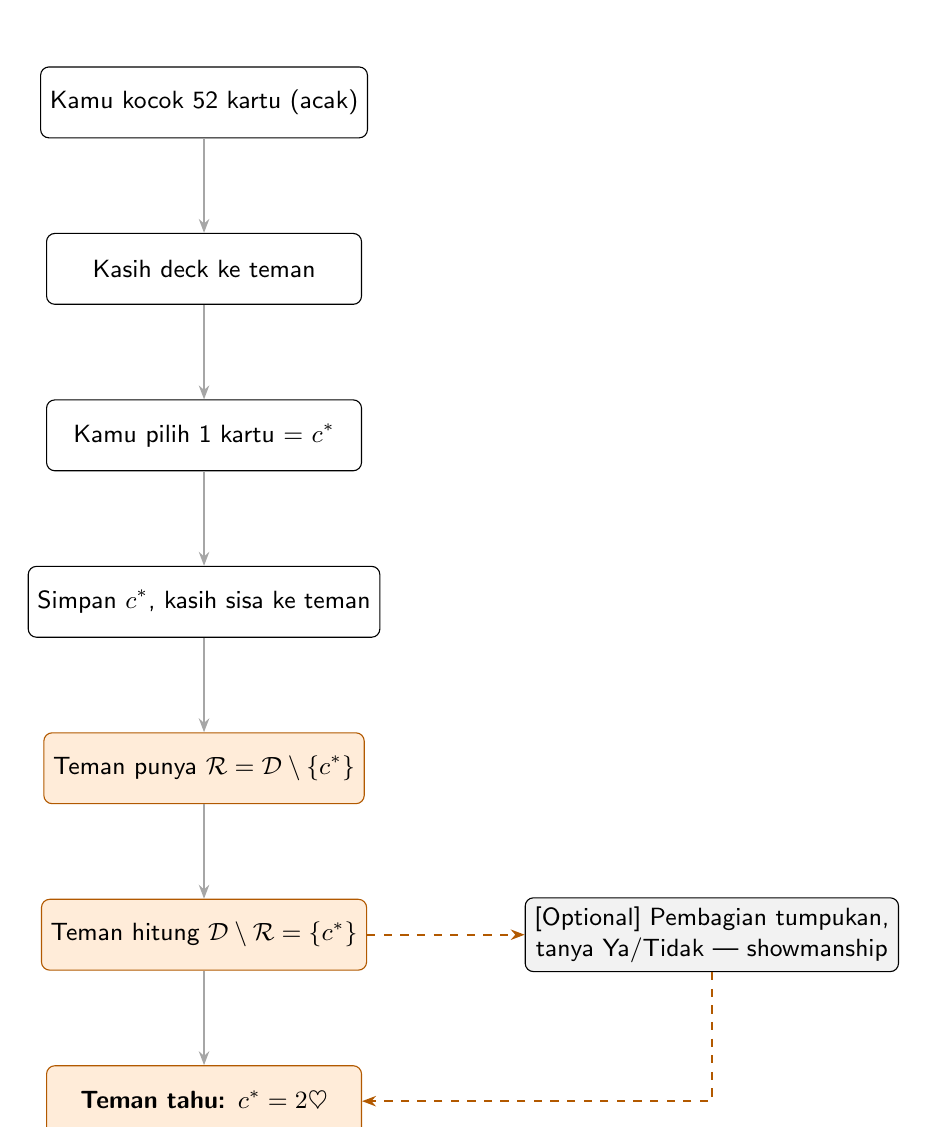
\begin{tikzpicture}[
    node distance=1.2cm,
    box/.style={draw, rounded corners=3pt, minimum width=4cm, minimum height=0.9cm, align=center, font=\small\sffamily},
    arr/.style={-{Stealth[length=5pt]}, thick, gray!70},
    hilite/.style={draw, rounded corners=3pt, minimum width=4cm, minimum height=0.9cm, align=center, font=\small\sffamily, fill=orange!15, draw=orange!70!black}
]
\node[box] (kocok) {Kamu kocok 52 kartu (acak)};
\node[box, below=of kocok] (kasih) {Kasih deck ke teman};
\node[box, below=of kasih] (pilih) {Kamu pilih 1 kartu = $c^*$};
\node[box, below=of pilih] (simpan) {Simpan $c^*$, kasih sisa ke teman};
\node[hilite, below=of simpan] (temanPunya) {Teman punya $\mathcal{R} = \mathcal{D} \setminus \{c^*\}$};
\node[hilite, below=of temanPunya] (hitung) {Teman hitung $\mathcal{D} \setminus \mathcal{R} = \{c^*\}$};
\node[hilite, below=of hitung] (tahu) {\textbf{Teman tahu: $c^* = 2\heartsuit$}};

\node[box, right=2cm of hitung, fill=gray!10] (show) {[Optional] Pembagian tumpukan,\\ tanya Ya/Tidak --- showmanship};

\draw[arr] (kocok) -- (kasih);
\draw[arr] (kasih) -- (pilih);
\draw[arr] (pilih) -- (simpan);
\draw[arr] (simpan) -- (temanPunya);
\draw[arr] (temanPunya) -- (hitung);
\draw[arr] (hitung) -- (tahu);
\draw[arr, dashed, orange!70!black] (hitung.east) -- (show.west);
\draw[arr, dashed, orange!70!black] (show.south) |- (tahu.east);
\end{tikzpicture}
\end{center}
\vspace{0.5em}

\textit{Box abu-abu = mekanisme asli identifikasi. Box oranye = langkah teatrikal opsional untuk showmanship.}

% =====================================================================
\section{Kesimpulan}
% =====================================================================

Tiga poin matematis yang harus kamu ingat:

\begin{enumerate}[label=\textbf{\arabic*.}, leftmargin=*]
    \item \textbf{Trik sebenarnya adalah operasi himpunan, bukan algoritma rumit.} Rumusnya cuma satu baris: $c^* = \mathcal{D} \setminus \mathcal{R}$.
    
    \item \textbf{Pembagian tumpukan dan pertanyaan Ya/Tidak adalah ``show'' bukan ``substance''.} Temanmu mengaku sendiri: ``tanpa gua bagi2 in gua juga bisa langsung tau kartu lu'' --- pernyataan ini benar secara matematis.
    
    \item \textbf{Sistem deterministik 100\%.} Tidak ada keberuntungan. Selama $\mathcal{D}$ diketahui dan $\mathcal{R}$ terobservasi, $c^*$ pasti teridentifikasi. Itu sebabnya trik ini disebut \emph{Sistem Deterministik} dalam matematika.
\end{enumerate}

Jadi, saat temanmu membagi-bagi kartu dan bertanya Ya/Tidak sampai sisa 3, sebenarnya ia hanya \textbf{membeli waktu} supaya trik terlihat seperti sulap. Kartumu sudah ia ketahui sejak detik pertama ia menerima sisa deck darimu.

\vspace{1em}
\begin{center}
\Large\bfseries $c^* = \mathcal{D} \setminus \mathcal{R}$ \\[0.3em]
\normalsize \emph{Itulah seluruh rahasianya.}
\end{center}

\end{document}
